\documentclass[11pt,a4paper]{article}

% ==============================================================================
% MASTER IOT LABORATORY PRACTICAL MANUAL & RECORD (COMPLETE UNABRIDGED EDITION)
% Strict Monochrome Minimalist Engineering Style (Modeled after DAA Practical)
% Comprehensive Theory, Equations, Architecture, Code, Data, and Analysis
% Includes Complete Assembly & Practical Record Attachment Reference Indicators
% ==============================================================================
\usepackage[utf8]{inputenc}
\usepackage[T1]{fontenc}
\usepackage{lmodern}
\usepackage[left=2.0cm, right=2.0cm, top=2.0cm, bottom=2.0cm]{geometry}
\usepackage{setspace}
\setstretch{1.08}
\usepackage{amsmath,amssymb,amsfonts,amsthm}
\usepackage{graphicx}
\usepackage{listings}
\usepackage{tcolorbox}
\tcbuselibrary{skins,breakable,listings}
\usepackage{tikz}
\usepackage{circuitikz}
\usetikzlibrary{shapes.geometric,arrows.meta,positioning,trees,calc}
\usepackage{booktabs}
\usepackage{tabularx}
\usepackage{array}
\usepackage{titlesec}
\usepackage{enumitem}
\usepackage{hyperref}
\usepackage{caption}
\captionsetup{font=small, labelfont=bf, justification=centering}
\usepackage{microtype}
\usepackage{float}

% Clean Minimal Page Numbering
\pagestyle{plain}

\hypersetup{
    hidelinks,
    pdfauthor={Department of Computer Science \& Engineering},
    pdftitle={Internet of Things (IoT) Laboratory Practical Record & Assembly Manual},
    pdfsubject={Comprehensive IoT Practical Manual & Assembly Guide for CSE}
}

% Classic Engineering Typographic Section Formatting
\titleformat{\section}
  {\normalfont\Large\bfseries}{\thesection}{1em}{}[\titlerule]
\titleformat{\subsection}
  {\normalfont\large\bfseries}{\thesubsection}{0.8em}{}
\titleformat{\subsubsection}
  {\normalfont\normalsize\bfseries\itshape}{\thesubsubsection}{0.6em}{}

\titlespacing*{\section}{0pt}{14pt}{6pt}
\titlespacing*{\subsection}{0pt}{10pt}{5pt}
\titlespacing*{\subsubsection}{0pt}{8pt}{4pt}

% Pure Black & White Sharp Box Containers
\newtcolorbox{bwcard}[1][]{
    enhanced,
    sharp corners,
    colback=white,
    colframe=black,
    boxrule=0.8pt,
    top=6pt, bottom=6pt, left=8pt, right=8pt,
    #1
}

\newtcolorbox{infobox}[1][]{
    enhanced,
    sharp corners,
    colback=white,
    colframe=black,
    boxrule=0.8pt,
    top=5pt, bottom=5pt, left=7pt, right=7pt,
    #1
}

% Sleek Attachment Callout Box
\newtcolorbox{attachmentbox}[1][]{
    enhanced,
    sharp corners,
    colback=gray!5,
    colframe=black,
    boxrule=1.0pt,
    top=5pt, bottom=5pt, left=8pt, right=8pt,
    #1
}

% Listings Styling (Strict Monochrome)
\lstdefinestyle{bwArduino}{
    language=C++,
    basicstyle=\ttfamily\footnotesize,
    keywordstyle=\bfseries,
    commentstyle=\itshape,
    stringstyle=\ttfamily,
    numbers=left,
    numberstyle=\tiny,
    numbersep=6pt,
    stepnumber=1,
    breaklines=true,
    breakatwhitespace=true,
    frame=single,
    rulecolor=\color{black},
    tabsize=2,
    showstringspaces=false,
    columns=fullflexible,
    keepspaces=true,
    aboveskip=6pt,
    belowskip=6pt
}

\lstdefinestyle{bwTerminal}{
    basicstyle=\ttfamily\footnotesize,
    numbers=none,
    breaklines=true,
    breakatwhitespace=true,
    frame=single,
    rulecolor=\color{black},
    columns=fullflexible,
    keepspaces=true,
    aboveskip=6pt,
    belowskip=6pt
}

\begin{document}

% ==============================================================================
% TITLE & CONTINUOUS EVALUATION RECORD INDEX
% ==============================================================================
\begin{center}
    {\LARGE\bfseries INTERNET OF THINGS (IoT) LABORATORY}\\[0.15cm]
    {\large\bfseries MASTER PRACTICAL MANUAL \& COMPLETE LABORATORY RECORD}\\[0.20cm]
    {\normalsize\textbf{Department of Computer Science and Engineering / Information Technology}}\\[0.08cm]
    {\footnotesize\textbf{Academic Session: 2025--2026 \quad $\bullet$ \quad Degree: Bachelor of Technology (B.Tech)}}
\end{center}
\vspace{-0.2cm}
\rule{\textwidth}{1.2pt}
\vspace{0.25cm}

\subsection*{Laboratory Continuous Evaluation Matrix}
\begin{center}
\small
\renewcommand{\arraystretch}{1.25}
\begin{tabularx}{\textwidth}{|c|X|c|c|c|c|}
\hline
\textbf{Exp No.} & \textbf{Experiment Title} & \textbf{Date of Exp.} & \textbf{Date of Sub.} & \textbf{Max Marks (10)} & \textbf{Faculty Sign} \\
\hline
\textbf{01} & Study of IoT Architecture, Characteristics, Multi-Tier Protocol Stack \& Constrained Standards & & & & \\
\hline
\textbf{02} & Arduino UNO Hardware Architecture \& Dual Alternating LED Interfacing with Current-Limiting Derivations & & & & \\
\hline
\textbf{03} & DHT11 Digital Sensor Interfacing, 1-Wire Protocol Decoding \& Closed-Loop Temperature Alert System & & & & \\
\hline
\end{tabularx}
\end{center}

\vspace{0.15cm}
\subsection*{Practical Copy Assembly \& Diagram Attachment Mapping Guide}
\begin{attachmentbox}
\footnotesize
\textbf{Assembly Instructions for Students:}
\begin{enumerate}[noitemsep, leftmargin=*]
    \item \textbf{Right-Hand Ruled Pages:} Handwrite the Aim, Apparatus, Detailed Theory, Equations, Step-by-Step Algorithms, Code Explanations, Results, and Viva-Voce answers from the \textit{Handwritten Practical Record Guide} (\texttt{IOT\_Handwritten\_Theory\_Guide.pdf}).
    \item \textbf{Left-Hand Unruled / Blank Pages:} Print the 6 sheets of the \textit{Printable Attachments Booklet} (\texttt{IOT\_Printable\_Diagrams\_and\_Codes.pdf}) and paste each corresponding sheet opposite the written experiment text according to the master mapping table below:
\end{enumerate}

\vspace{0.1cm}
\renewcommand{\arraystretch}{1.2}
\begin{tabularx}{\linewidth}{|c|p{4.2cm}|p{3.8cm}|X|}
\hline
\textbf{Exp.} & \textbf{Handwritten Section (Right Page)} & \textbf{Printable PDF Attachment} & \textbf{Attachment Contents} \\
\hline
\textbf{Exp 1} & Overview \& 5-Tier Architecture & \textbf{Sheet 1 (Page 1)} & Figure 1.1 (5-Tier Architecture) \& Table 1.1 (Protocols) \\
\textbf{Exp 2} & Arduino Architecture \& Circuits & \textbf{Sheet 2 (Page 2)} & Figure 2.1 (Board Photo), Fig 2.2 (Fritzing), Fig 2.3 (Schematic), Table 2.1 (Pins) \\
\textbf{Exp 2} & Firmware Execution \& Logic & \textbf{Sheet 3 (Page 3)} & Program Listing 2.1 (C++ Code), Fig 2.4 (Waveforms), Table 2.2 (Truth Table) \\
\textbf{Exp 3} & 1-Wire Handshake \& Sensor Wiring & \textbf{Sheet 4 (Page 4)} & Figure 3.1 (Handshake Timing), Fig 3.2 (Fritzing), Fig 3.3 (Schematic), Table 3.1 \\
\textbf{Exp 3} & DHT11 Firmware Implementation & \textbf{Sheet 5 (Page 5)} & Program Listing 3.1 (Complete C++ Telemetry \& Alert Code) \\
\textbf{Exp 3} & Telemetry Logs \& Serial Stream & \textbf{Sheet 6 (Page 6)} & Table 3.2 (Telemetry Observations Log) \& Serial Monitor Output Capture \\
\hline
\end{tabularx}
\end{attachmentbox}

\newpage

% ==============================================================================
% EXPERIMENT 01: OVERVIEW OF IOT
% ==============================================================================
\section{Experiment 01: Overview of IoT Architecture, Characteristics \& Protocols}

\subsection{Aim \& Objectives}
\begin{itemize}[noitemsep]
    \item To understand the foundational architecture and engineering concepts of the Internet of Things (IoT).
    \item To systematically analyze the ten core characteristics defining modern cyber-physical IoT ecosystems.
    \item To study the 5-tier hierarchical IoT architectural reference framework from physical environment to cloud application.
    \item To compare and contrast constrained application layer communication protocols (MQTT, CoAP, HTTP/REST, WebSockets).
\end{itemize}

\subsection{Theoretical Background \& Principles}

\subsubsection{Formal Definitions and Conceptual Paradigm}
The term \textbf{Internet of Things (IoT)} was first coined in 1999 by Kevin Ashton during work at the MIT Auto-ID Center. Standardizing bodies define IoT as follows:
\begin{itemize}[noitemsep]
    \item \textbf{ITU-T (Recommendation Y.2060):} \textit{``A dynamic global network infrastructure with self-configuring capabilities based on standard and interoperable communication protocols where physical and virtual `things' have identities, physical attributes, and virtual personalities, use intelligent interfaces, and are seamlessly integrated into the information network.''}
    \item \textbf{IEEE IoT Working Group:} \textit{``A network of items—each embedded with sensors—which are connected to the Internet, enabling physical objects to collect and exchange data without requiring human-to-human or human-to-computer interaction.''}
\end{itemize}

At its core, IoT bridges the cyber-physical divide: real-world continuous physical parameters (temperature, light, vibration, moisture) are captured by \textbf{sensors (transducers)}, converted into electrical signals, digitized by \textbf{microcontrollers (edge compute nodes)}, transmitted over \textbf{communication networks}, processed by \textbf{cloud/fog analytics engines}, and translated into autonomous physical actions via \textbf{actuators}.

\subsubsection{Detailed Examination of the Ten Core Characteristics of IoT}
\begin{enumerate}[leftmargin=*]
    \item \textbf{Interconnectivity \& Global Addressing:} Any physical object with an integrated sensing or actuating unit can be assigned a unique logical address (IPv6 / 6LoWPAN) and integrated into the global communication infrastructure.
    \item \textbf{Things-Related Services \& Virtual Digital Twins:} The IoT provides domain-specific semantic services between physical devices and their virtual software representations (digital twins) in cloud platforms.
    \item \textbf{Heterogeneity across Hardware \& Software:} Interoperability across 8-bit MCUs (ATmega328P), 32-bit SoCs (ESP32, ARM Cortex-M), diverse RTOS environments (FreeRTOS, Zephyr), and multi-vendor fieldbuses.
    \item \textbf{Dynamic Changes in State \& Context Awareness:} IoT nodes dynamically alternate between deep-sleep modes ($<15\,\mu\text{A}$) and active radio bursts, adapting to fluctuating network topologies and battery levels.
    \item \textbf{Massive Scale \& Concurrency:} Networks handle orders of magnitude more connected endpoints than the human Internet, requiring non-blocking asynchronous brokers (e.g., MQTT Mosquitto, EMQX).
    \item \textbf{Embedded Edge Intelligence \& Fog Computing:} Offloading data preprocessing, filtering, and inference to local microcontrollers reduces bandwidth consumption, network egress costs, and cloud latency.
    \item \textbf{Autonomous Self-Configuration and Self-Healing:} Mesh networks (Zigbee, RPL) dynamically re-route data packets around failing nodes, while FOTA delivers cryptographic binary updates.
    \item \textbf{Open Standards \& Protocol Interoperability:} Conformance to vendor-neutral global standards (IEEE 802.15.4, RFC 7252 CoAP, OASIS MQTT, ISO/IEC) ensures universal data exchange across heterogeneous systems.
    \item \textbf{End-to-End Cryptographic Security:} Implementing the CIA Triad (Confidentiality, Integrity, Availability) on constrained hardware using hardware-accelerated AES-128/256, Elliptic Curve Cryptography (ECC), and TLS/DTLS.
    \item \textbf{Data-Driven Value Creation:} The ultimate objective of an IoT network is the extraction of actionable predictive analytics, anomaly detection, and operational automation via Kafka, InfluxDB, and ML pipelines.
\end{enumerate}

\begin{attachmentbox}
\footnotesize
\textbf{[ $\hookrightarrow$ Practical Record Attachment Reference for Experiment 1 ]}\\
Paste \textbf{Sheet 1 (Page 1)} from \texttt{IOT\_Printable\_Diagrams\_and\_Codes.pdf} on the \textbf{Left-Hand Blank Page} opposite this theory section. It contains \textbf{Figure 1.1} (5-Tier Architecture) and \textbf{Table 1.1} (Constrained Protocols Comparison).
\end{attachmentbox}

\subsection{5-Tier Hierarchical IoT Architecture Framework}
Modern enterprise and industrial IoT systems are structured into a 5-tier hierarchical architectural model:

\begin{figure}[H]
\centering
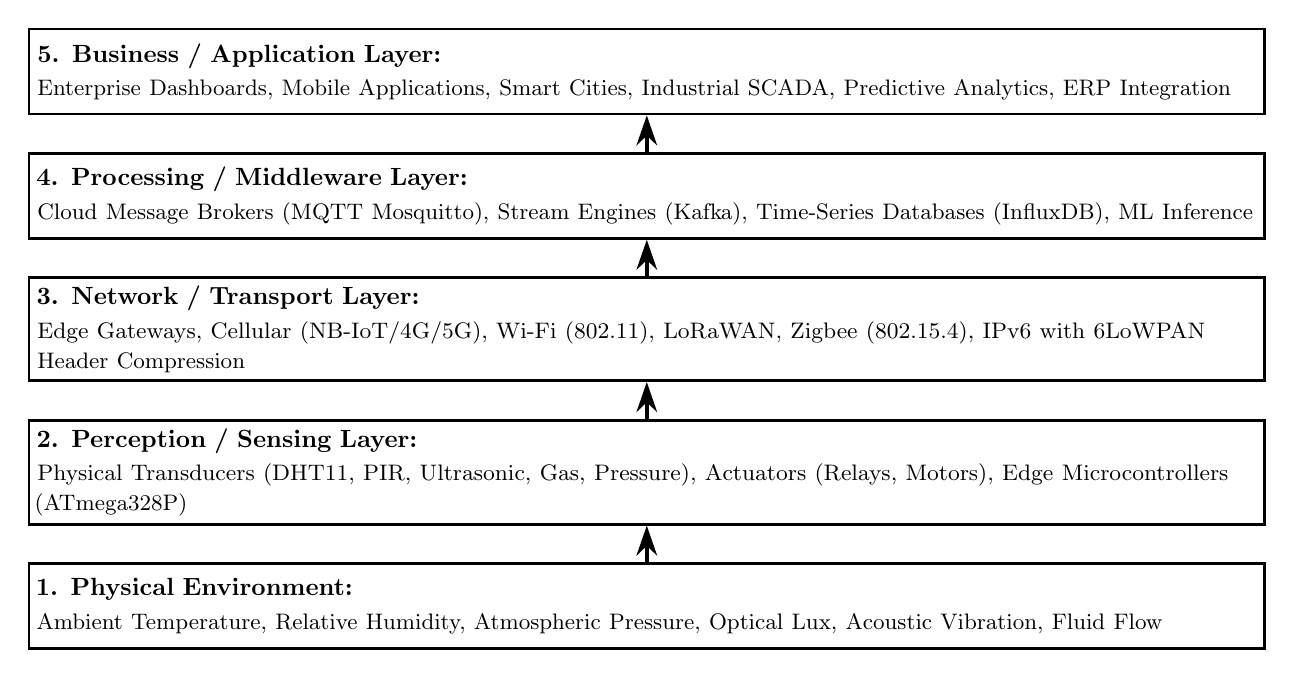
\begin{tikzpicture}[scale=0.90, every node/.style={transform shape}]
    \tikzstyle{layer} = [rectangle, draw=black, fill=white, line width=1.0pt, text width=17.2cm, minimum height=1.20cm, font=\normalsize, align=left]
    \tikzstyle{arr} = [ultra thick, -{Stealth[length=3.8mm, width=2.6mm]}, draw=black]

    \node [layer] (l5) {\textbf{5. Business / Application Layer:}\\[0.05cm] \small Enterprise Dashboards, Mobile Applications, Smart Cities, Industrial SCADA, Predictive Analytics, ERP Integration};
    \node [layer, below=0.52cm of l5] (l4) {\textbf{4. Processing / Middleware Layer:}\\[0.05cm] \small Cloud Message Brokers (MQTT Mosquitto), Stream Engines (Kafka), Time-Series Databases (InfluxDB), ML Inference};
    \node [layer, below=0.52cm of l4] (l3) {\textbf{3. Network / Transport Layer:}\\[0.05cm] \small Edge Gateways, Cellular (NB-IoT/4G/5G), Wi-Fi (802.11), LoRaWAN, Zigbee (802.15.4), IPv6 with 6LoWPAN Header Compression};
    \node [layer, below=0.52cm of l3] (l2) {\textbf{2. Perception / Sensing Layer:}\\[0.05cm] \small Physical Transducers (DHT11, PIR, Ultrasonic, Gas, Pressure), Actuators (Relays, Motors), Edge Microcontrollers (ATmega328P)};
    \node [layer, below=0.52cm of l2] (l1) {\textbf{1. Physical Environment:}\\[0.05cm] \small Ambient Temperature, Relative Humidity, Atmospheric Pressure, Optical Lux, Acoustic Vibration, Fluid Flow};

    \draw [arr] (l1.north) -- (l2.south);
    \draw [arr] (l2.north) -- (l3.south);
    \draw [arr] (l3.north) -- (l4.south);
    \draw [arr] (l4.north) -- (l5.south);
\end{tikzpicture}
\caption{5-Tier Hierarchical IoT Architecture Reference Framework.}
\label{fig:iot_architecture}
\end{figure}

\subsubsection{Architectural Layer Descriptions}
\begin{itemize}[leftmargin=*]
    \item \textbf{Perception Layer:} The physical interface to the real world. Transducers convert physical phenomena into electrical signals (analog voltage or digital data). Microcontrollers sample, condition, and packetize these signals.
    \item \textbf{Network Layer:} Responsible for secure, reliable transmission of sensor packets across local networks and the Internet to cloud endpoints. Utilizes low-power wireless personal area networks (WPAN) and LPWAN technologies.
    \item \textbf{Processing Layer:} Ingests millions of concurrent sensor messages, performs authentication, validates checksums, stores historical telemetry in time-series databases, and runs automated analytics algorithms.
    \item \textbf{Application Layer:} Provides user-facing interfaces, visual graphs, automated threshold alarms, control commands, and API integrations with external enterprise applications.
\end{itemize}

\subsection{Constrained Communication Protocols Analysis}
Traditional Internet protocols like HTTP/1.1 are excessively heavy for battery-operated microcontrollers due to large text headers, connection overhead, and synchronous polling. IoT employs specialized protocols:

\begin{table}[H]
\centering
\small
\renewcommand{\arraystretch}{1.3}
\begin{tabularx}{\textwidth}{|p{2.1cm}|p{2.0cm}|p{3.1cm}|p{2.0cm}|X|}
\hline
\textbf{Protocol} & \textbf{Transport} & \textbf{Messaging Model} & \textbf{Header Size} & \textbf{Primary Application Domain} \\
\hline
\textbf{MQTT} & TCP (1883) & Publish / Subscribe & 2 Bytes (Fixed) & Real-time sensor telemetry, SCADA, battery-backed nodes. \\
\textbf{CoAP} & UDP (5683) & REST Request / Response & 4 Bytes (Fixed) & Constrained 8-bit MCUs, low-power lossy networks (LLNs). \\
\textbf{HTTP/REST} & TCP (80/443) & Client / Server Request & $>500$ B (Text) & Cloud-to-cloud APIs, enterprise REST integrations. \\
\textbf{WebSocket} & TCP (80) & Full-Duplex Stream & 2--10 B (Binary) & Live browser telemetry monitoring dashboards. \\
\hline
\end{tabularx}
\caption{Comparison of Constrained Application Protocols in IoT Systems.}
\label{tab:protocols}
\end{table}

\subsubsection{MQTT Architecture and Quality of Service (QoS) Levels}
MQTT operates on a decoupled client-broker topology:
\begin{itemize}[noitemsep]
    \item \textbf{QoS 0 (At most once):} Messages are dispatched without acknowledgment (Fire and Forget). Minimum overhead, but messages may be lost over unstable networks.
    \item \textbf{QoS 1 (At least once):} The publisher expects a `PUBACK` confirmation from the broker. If unacknowledged within a timeout, the message is retransmitted (duplicate delivery possible).
    \item \textbf{QoS 2 (Exactly once):} A four-step handshake (`PUBLISH` $\rightarrow$ `PUBREC` $\rightarrow$ `PUBREL` $\rightarrow$ `PUBCOMP`) guarantees that every message arrives exactly once without duplication.
\end{itemize}

\subsection{Discussion \& Analytical Review}
\begin{itemize}[noitemsep]
    \item \textbf{Trade-Off Between Range and Throughput:} Technologies like LoRaWAN achieve ultra-long communication range ($>10\text{ km}$) and $5-10$ year battery life by operating at narrow bandwidths and low data rates ($0.3-50\text{ kbps}$), whereas Wi-Fi delivers high bandwidth ($>100\text{ Mbps}$) at the cost of high power consumption.
    \item \textbf{Security Vulnerabilities in Constrained Nodes:} 8-bit microcontrollers often lack dedicated hardware acceleration for asymmetric cryptography (RSA/ECC), making them vulnerable to man-in-the-middle attacks unless paired with secure hardware elements (e.g., ATECC608A).
\end{itemize}

\subsection{Viva-Voce Questions \& Detailed Answers}
\begin{enumerate}[leftmargin=*]
    \item \textbf{Q: What is the primary difference between MQTT and CoAP?}\\
    \textbf{Ans:} MQTT is a broker-centric publish/subscribe protocol operating over connection-oriented TCP, ideal for continuous telemetry streams. CoAP is a client-server RESTful protocol operating over connectionless UDP datagrams, optimized for sleeping nodes that periodically wake up to transmit a packet.
    \item \textbf{Q: What is the role of 6LoWPAN in the IoT protocol stack?}\\
    \textbf{Ans:} 6LoWPAN (IPv6 over Low-Power Wireless Personal Area Networks) implements header compression and packet fragmentation algorithms to fit standard 128-bit IPv6 packets into small IEEE 802.15.4 link-layer frames (which have a maximum payload of 127 bytes).
    \item \textbf{Q: What is the purpose of an IoT Gateway?}\\
    \textbf{Ans:} An IoT Gateway bridges short-range, non-IP fieldbus networks (Zigbee, BLE, Modbus) with IP-based enterprise networks and the Internet, performing protocol translation, data aggregation, local filtering, and encryption.
\end{enumerate}

\newpage

% ==============================================================================
% EXPERIMENT 02: ARDUINO UNO & DUAL LED INTERFACING
% ==============================================================================
\section{Experiment 02: Arduino UNO Hardware Architecture \& Dual LED Interfacing}

\subsection{Aim \& Objectives}
\begin{itemize}[noitemsep]
    \item To systematically study the hardware subsystems, pinout configuration, memory structure, and power management of the Arduino UNO development board.
    \item To interface two discrete LEDs (Green and Red) to GPIO Pins D8 and D7 using a solderless breadboard.
    \item To mathematically derive the required current-limiting resistor values using Ohm's Law and LED semiconductor forward voltage characteristics.
    \item To develop, flash, and verify an Arduino C++ program that drives the two LEDs in strict anti-phase alternating blinking at $1.0\,\text{s}$ intervals.
\end{itemize}

\subsection{Hardware Apparatus \& Bill of Materials}
\begin{table}[H]
\centering
\footnotesize
\renewcommand{\arraystretch}{1.25}
\begin{tabularx}{\textwidth}{|c|l|X|c|}
\hline
\textbf{S.No.} & \textbf{Component / Apparatus} & \textbf{Technical Specification} & \textbf{Quantity} \\
\hline
1 & Arduino UNO R3 Development Board & ATmega328P MCU, 16 MHz Crystal, 5V Logic, 32 KB Flash & 1 unit \\
2 & Green LED ($5\,\text{mm}$) & Gallium Phosphide (GaP), $\lambda \approx 525\,\text{nm}$, $V_F \approx 2.1\,\text{V}$, $I_{\max} = 20\,\text{mA}$ & 1 unit \\
3 & Red LED ($5\,\text{mm}$) & Gallium Arsenide Phosphide (GaAsP), $\lambda \approx 625\,\text{nm}$, $V_F \approx 1.9\,\text{V}$ & 1 unit \\
4 & Carbon Film Resistors & $1\,\text{k}\Omega$ (or $220\,\Omega$), $0.25\,\text{W}$ Rating, $\pm 5\%$ Tolerance & 2 units \\
5 & Solderless Breadboard & Standard 830 Tie-point Breadboard with Power Rails & 1 unit \\
6 & Jumper Wires & 24 AWG Solid Core Male-to-Male Wires & 4 units \\
7 & USB Programming Cable & USB Type-A to Type-B Cable ($1.0\,\text{m}$) & 1 unit \\
\hline
\end{tabularx}
\caption{Apparatus and Bill of Materials for Experiment 2.}
\label{tab:exp2_bom}
\end{table}

\begin{attachmentbox}
\footnotesize
\textbf{[ $\hookrightarrow$ Practical Record Attachment Reference for Experiment 2 (Hardware) ]}\\
Paste \textbf{Sheet 2 (Page 2)} from \texttt{IOT\_Printable\_Diagrams\_and\_Codes.pdf} on the \textbf{Left-Hand Blank Page} opposite this hardware section. It contains \textbf{Figure 2.1} (Arduino Board Photo), \textbf{Figure 2.2} (Breadboard Fritzing), \textbf{Figure 2.3} (CircuiTikZ Schematic), and \textbf{Table 2.1} (Pin Matrix).
\end{attachmentbox}

\subsection{Arduino UNO R3 Board Hardware Architecture}
The Arduino UNO R3 is an open-source microcontroller board built around the Microchip ATmega328P 8-bit AVR RISC microcontroller.

\begin{figure}[H]
\centering
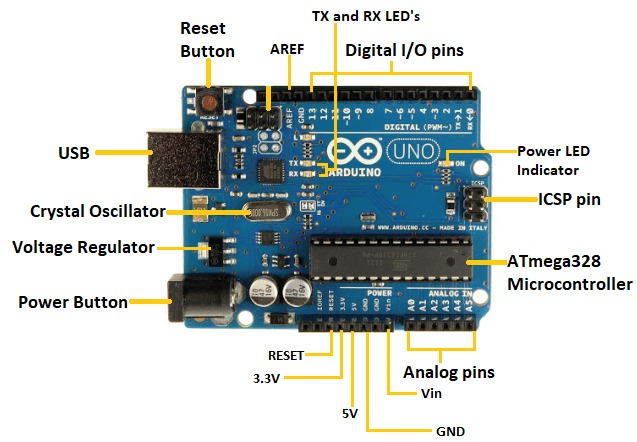
\includegraphics[width=0.68\textwidth]{Arduino Board Configuration.jpg}
\caption{Arduino UNO R3 Board Hardware Layout and Pin Configuration.}
\label{fig:arduino_board_layout}
\end{figure}

\subsubsection{Detailed Hardware Subsystems Analysis}
\begin{enumerate}[leftmargin=*]
    \item \textbf{ATmega328P Microcontroller Core:}
    \begin{itemize}[noitemsep]
        \item \textbf{Architecture:} 8-bit AVR Harvard RISC architecture executing single-cycle instructions up to 16 MIPS at 16 MHz.
        \item \textbf{Flash Memory:} 32 KB on-chip in-system self-programmable Flash memory (0.5 KB utilized by the Optiboot bootloader).
        \item \textbf{SRAM:} 2 KB internal static RAM for dynamic variable allocation and call stacks.
        \item \textbf{EEPROM:} 1 KB non-volatile byte-addressable memory with 100,000 write cycle endurance.
    \end{itemize}
    \item \textbf{Digital I/O Subsystem (Pins D0--D13):}
    \begin{itemize}[noitemsep]
        \item 14 digital input/output pins. Each pin can source or sink a nominal current of $20\text{ mA}$ (absolute maximum limit: $40\text{ mA}$).
        \item \textbf{PWM Channels:} Pins 3, 5, 6, 9, 10, and 11 provide 8-bit hardware Pulse Width Modulation (PWM) at $\approx 490\,\text{Hz}$ or $980\,\text{Hz}$.
        \item \textbf{UART Interface:} Pins D0 (RX) and D1 (TX) connect to the hardware serial bus.
        \item \textbf{SPI Interface:} Pin 10 (SS), Pin 11 (MOSI), Pin 12 (MISO), Pin 13 (SCK).
    \end{itemize}
    \item \textbf{Analog Input Subsystem (Pins A0--A5):}
    \begin{itemize}[noitemsep]
        \item 6 analog input channels connected to an internal 10-bit Successive Approximation Analog-to-Digital Converter (ADC).
        \item Resolves voltages from $0\,\text{V}$ to $5.0\,\text{V}$ into integer values from $0$ to $1023$, yielding a voltage resolution of $Q = \frac{5.0\,\text{V}}{1024} = 4.88\,\text{mV/count}$.
    \end{itemize}
    \item \textbf{Clock and Reset Subsystem:}
    \begin{itemize}[noitemsep]
        \item \textbf{Crystal Oscillator:} 16 MHz external ceramic resonator/crystal provides a system clock period of $T_{\text{clk}} = \frac{1}{16\,\text{MHz}} = 62.5\,\text{ns}$.
        \item \textbf{Reset Push Button:} Pulls the active-LOW $\overline{\text{RESET}}$ pin to ground to restart program execution from address \texttt{0x0000}.
    \end{itemize}
    \item \textbf{Power Distribution and Voltage Regulation:}
    \begin{itemize}[noitemsep]
        \item \textbf{DC Power Jack:} Accepts $7-12\,\text{V}$ unregulated DC input, regulated down to $5\,\text{V}$ via an onboard NCP1117ST50 linear regulator.
        \item \textbf{USB Supply Protection:} Equipped with a $500\text{ mA}$ resettable polyfuse to safeguard the host PC USB port against short circuits.
        \item \textbf{3.3V Output:} Onboard LP2985 low-dropout regulator supplies up to $150\text{ mA}$ at $3.3\,\text{V}$.
    \end{itemize}
\end{enumerate}

\subsection{Theoretical Principles \& Mathematical Derivations}

\subsubsection{Semiconductor Physics of Light Emitting Diodes (LEDs)}
A Light Emitting Diode is a heavily doped $P$-$N$ junction diode fabricated from direct bandgap compound semiconductors. When forward-biased, minority electrons from the $N$-region and holes from the $P$-region are injected across the depletion zone. Recombination releases energy as emitted photons:
\begin{equation}
E_g = h \cdot \nu = \frac{h \cdot c}{\lambda}
\end{equation}
Where $E_g$ is the bandgap energy, $h = 6.626 \times 10^{-34}\,\text{J}\cdot\text{s}$, and $c = 3.0 \times 10^8\,\text{m/s}$.

\subsubsection{Ohm's Law Derivation for Current-Limiting Resistor}
Applying Kirchhoff's Voltage Law (KVL) around the closed GPIO-to-Ground output loop:
\begin{equation}
V_{CC} - V_R - V_F = 0 \implies R = \frac{V_{CC} - V_F}{I_F}
\end{equation}
Given $V_{CC} = 5.0\,\text{V}$, $V_F \approx 2.0\,\text{V}$, and safe target current $I_F = 15\,\text{mA}$:
\begin{equation}
R_{\text{calculated}} = \frac{5.0\,\text{V} - 2.0\,\text{V}}{0.015\,\text{A}} = \frac{3.0\,\text{V}}{0.015\,\text{A}} = 200\,\Omega
\end{equation}
Evaluating standard commercial resistor selections:
\begin{itemize}[noitemsep]
    \item \textbf{Using $R = 220\,\Omega$:} $I_F = \frac{5.0\,\text{V} - 2.0\,\text{V}}{220\,\Omega} = 13.63\,\text{mA}$ (Maximum safe brightness).
    \item \textbf{Using $R = 1\,\text{k}\Omega$:} $I_F = \frac{5.0\,\text{V} - 2.0\,\text{V}}{1000\,\Omega} = 3.0\,\text{mA}$ (Conservative low-power drive).
    \item \textbf{Power Dissipation:} $P_R = I_F^2 \cdot R = (0.003\,\text{A})^2 \cdot 1000\,\Omega = 9\,\text{mW} \ll 0.25\,\text{W}$ (Safe margin).
\end{itemize}

\subsection{Breadboard Interfacing \& Circuit Schematics}
\begin{figure}[H]
\centering
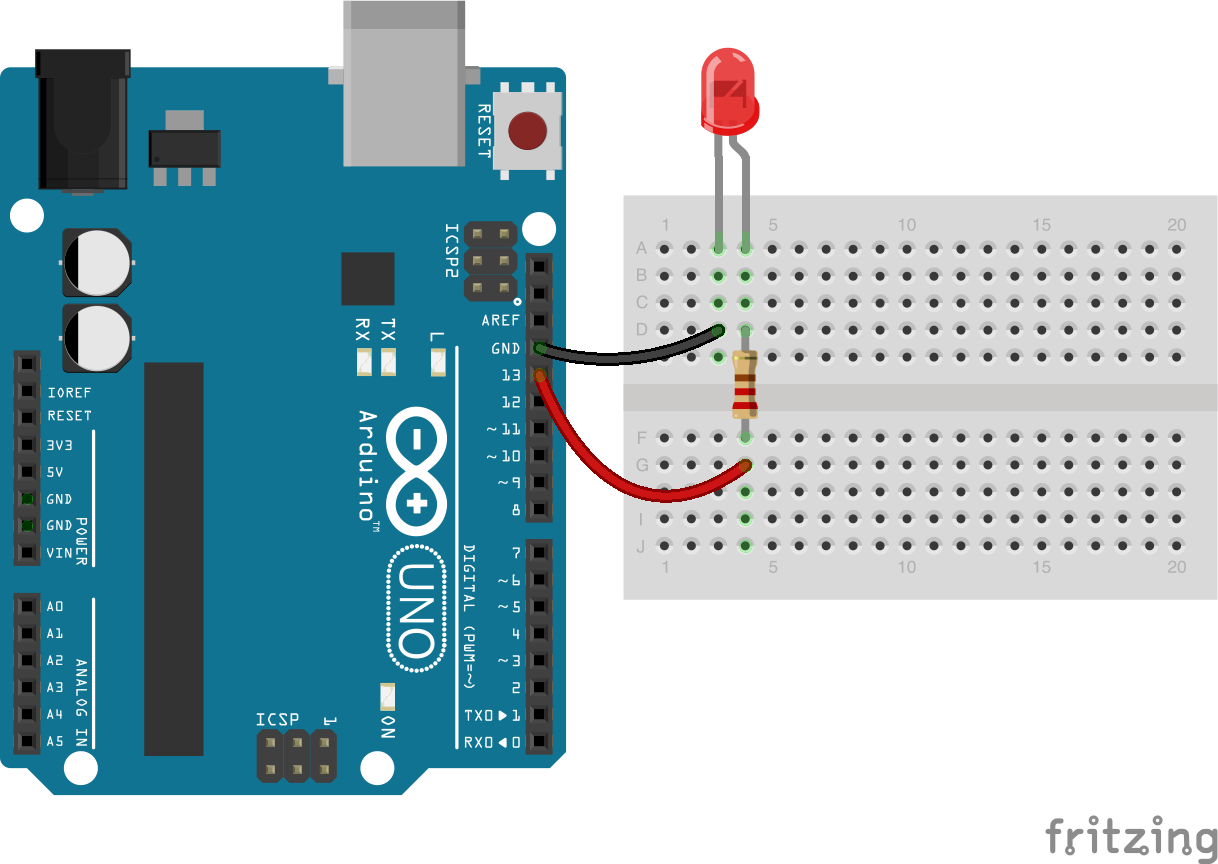
\includegraphics[height=3.8cm, keepaspectratio]{led_resistor.png}
\caption{Breadboard Fritzing Wiring Diagram for LED Interfacing.}
\label{fig:led_breadboard}
\end{figure}

\begin{figure}[H]
\centering
\begin{circuitikz}[american, scale=0.74]
    \draw[fill=white, draw=black, line width=1.0pt] (0,0) rectangle (4.2,3.8);
    \node at (2.1,3.3) [font=\bfseries\small] {ARDUINO UNO};
    
    \node (p8) at (4.2,2.6) [anchor=east, font=\small\bfseries] {D8 (Pin 8)};
    \node (p7) at (4.2,1.5) [anchor=east, font=\small\bfseries] {D7 (Pin 7)};
    \node (gnd) at (4.2,0.5) [anchor=east, font=\small\bfseries] {GND};

    \draw (4.2,2.6) -- (5.2,2.6) to[R, l=$R_1(1\,\text{k}\Omega)$, *-] (7.2,2.6) to[leDo, -*] (9.2,2.6) -- (9.2,0.5);
    \node[right, font=\small\bfseries] at (9.3,2.6) {$\text{LED}_1\ (\text{Green})$};

    \draw (4.2,1.5) -- (5.2,1.5) to[R, l=$R_2(1\,\text{k}\Omega)$, *-] (7.2,1.5) to[leDo, -*] (9.2,1.5) -- (9.2,0.5);
    \node[right, font=\small\bfseries] at (9.3,1.5) {$\text{LED}_2\ (\text{Red})$};

    \draw (4.2,0.5) -- (9.2,0.5) node[ground]{};
\end{circuitikz}
\caption{Complete CircuiTikZ Schematic for Dual Alternating LED Interfacing.}
\label{fig:exp2_circuit}
\end{figure}

\subsection{Pin Interconnection Table}
\begin{table}[H]
\centering
\small
\renewcommand{\arraystretch}{1.22}
\begin{tabularx}{\textwidth}{|l|l|l|X|}
\hline
\textbf{Arduino Terminal} & \textbf{Breadboard Component} & \textbf{Component Terminal} & \textbf{Signal Function} \\
\hline
Digital Pin 8 (D8) & Resistor $R_1$ ($1\,\text{k}\Omega$) & Lead 1 & GPIO Push-Pull Output Channel 1 \\
Resistor $R_1$ ($1\,\text{k}\Omega$) & $\text{LED}_1$ (Green) & Anode (Long Leg, $+$) & Current-Limited 5V Drive ($I_{F1} \approx 3.0\text{ mA}$) \\
$\text{LED}_1$ (Green) & Common Ground Rail & Cathode (Flat Notch, $-$) & System Ground Return Path \\
\hline
Digital Pin 7 (D7) & Resistor $R_2$ ($1\,\text{k}\Omega$) & Lead 1 & GPIO Push-Pull Output Channel 2 \\
Resistor $R_2$ ($1\,\text{k}\Omega$) & $\text{LED}_2$ (Red) & Anode (Long Leg, $+$) & Current-Limited 5V Drive ($I_{F2} \approx 3.0\text{ mA}$) \\
$\text{LED}_2$ (Red) & Common Ground Rail & Cathode (Flat Notch, $-$) & System Ground Return Path \\
\hline
\end{tabularx}
\caption{Hardware Pin Wiring Interconnection Matrix for Experiment 2.}
\label{tab:exp2_pins}
\end{table}

\begin{attachmentbox}
\footnotesize
\textbf{[ $\hookrightarrow$ Practical Record Attachment Reference for Experiment 2 (Firmware \& Output) ]}\\
Paste \textbf{Sheet 3 (Page 3)} from \texttt{IOT\_Printable\_Diagrams\_and\_Codes.pdf} on the \textbf{Left-Hand Blank Page} opposite this firmware section. It contains \textbf{Program Listing 2.1} (Complete C++ Program), \textbf{Figure 2.4} (Timing Waveforms), and \textbf{Table 2.2} (Circuit Logic Truth Table).
\end{attachmentbox}

\subsection{Arduino C++ Firmware Implementation}
\begin{lstlisting}[style=bwArduino, caption={Arduino C++ Program for Dual Alternating LED Blinking.}]
/*
 * Experiment 02: Dual Alternating LED Interfacing with Arduino UNO
 * Hardware Pin Connections: Pin D8 -> Green LED | Pin D7 -> Red LED
 * Switching Interval: 1000 ms (1.0 second) Anti-Phase Blinking
 */

const int LED1_PIN = 8;    // Green LED Channel (Digital Pin 8)
const int LED2_PIN = 7;    // Red LED Channel (Digital Pin 7)
const unsigned long BLINK_INTERVAL = 1000; // Period: 1000 ms (1.0 s)

void setup() {
  // Configure both GPIO pins as digital output drivers
  pinMode(LED1_PIN, OUTPUT);
  pinMode(LED2_PIN, OUTPUT);
  
  // Set deterministic initial state (both OFF)
  digitalWrite(LED1_PIN, LOW);
  digitalWrite(LED2_PIN, LOW);
}

void loop() {
  // Phase 1: LED1 ON (Active HIGH), LED2 OFF (Active LOW)
  digitalWrite(LED1_PIN, HIGH);
  digitalWrite(LED2_PIN, LOW);
  delay(BLINK_INTERVAL);
  
  // Phase 2: LED1 OFF (Active LOW), LED2 ON (Active HIGH)
  digitalWrite(LED1_PIN, LOW);
  digitalWrite(LED2_PIN, HIGH);
  delay(BLINK_INTERVAL);
}
\end{lstlisting}

\subsection{Logic State Transitions \& Timing Waveforms}
\begin{figure}[H]
\centering
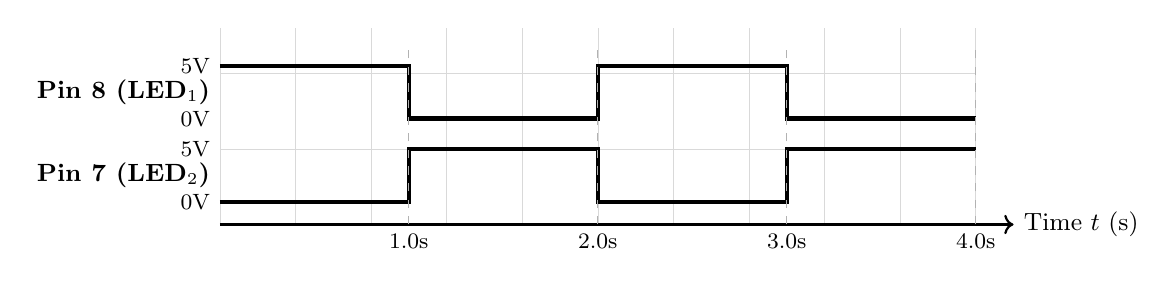
\begin{tikzpicture}[scale=0.96]
    \draw[step=1.0cm,gray!30,very thin] (0,0) grid (10,2.6);
    \draw[thick,->] (0,0) -- (10.5,0) node[right, font=\small] {Time $t$ (s)};
    
    % Pin 8 (LED1)
    \draw[ultra thick] (0,2.1) -- (2.5,2.1) -- (2.5,1.4) -- (5.0,1.4) -- (5.0,2.1) -- (7.5,2.1) -- (7.5,1.4) -- (10.0,1.4);
    \node[left, font=\small\bfseries] at (0,1.75) {Pin 8 ($\text{LED}_1$)};
    \node[left, font=\footnotesize] at (0,2.1) {5V};
    \node[left, font=\footnotesize] at (0,1.4) {0V};

    % Pin 7 (LED2)
    \draw[ultra thick] (0,0.3) -- (2.5,0.3) -- (2.5,1.0) -- (5.0,1.0) -- (5.0,0.3) -- (7.5,0.3) -- (7.5,1.0) -- (10.0,1.0);
    \node[left, font=\small\bfseries] at (0,0.65) {Pin 7 ($\text{LED}_2$)};
    \node[left, font=\footnotesize] at (0,1.0) {5V};
    \node[left, font=\footnotesize] at (0,0.3) {0V};
    
    \foreach \x/\t in {2.5/1.0s, 5.0/2.0s, 7.5/3.0s, 10.0/4.0s} {
        \draw[dashed, gray!60] (\x,0) -- (\x,2.4);
        \node[below, font=\footnotesize] at (\x,0) {\t};
    }
\end{tikzpicture}
\caption{Digital Logic Timing Waveforms for Anti-Phase Switching ($T = 1.0\,\text{s}$).}
\label{fig:exp2_waveform}
\end{figure}

\begin{table}[H]
\centering
\small
\renewcommand{\arraystretch}{1.3}
\begin{tabularx}{\textwidth}{|c|c|c|c|c|X|}
\hline
\textbf{Time Interval} & \textbf{Pin 8 Level} & \textbf{Pin 7 Level} & \textbf{$\text{LED}_1$ State} & \textbf{$\text{LED}_2$ State} & \textbf{Circuit Current \& Physical Observation} \\
\hline
$0.0\,\text{s} - 1.0\,\text{s}$ & HIGH ($5.0\,\text{V}$) & LOW ($0.0\,\text{V}$) & \textbf{ON} & \textbf{OFF} & $I_{F1} \approx 3.0\text{ mA}$; Green light emission active. \\
$1.0\,\text{s} - 2.0\,\text{s}$ & LOW ($0.0\,\text{V}$) & HIGH ($5.0\,\text{V}$) & \textbf{OFF} & \textbf{ON} & $I_{F2} \approx 3.0\text{ mA}$; Red light emission active. \\
$2.0\,\text{s} - 3.0\,\text{s}$ & HIGH ($5.0\,\text{V}$) & LOW ($0.0\,\text{V}$) & \textbf{ON} & \textbf{OFF} & State repeats in strict periodic anti-phase. \\
\hline
\end{tabularx}
\caption{Circuit Logic Truth Table and Operational States.}
\label{tab:exp2_truth}
\end{table}

\subsection{Discussion \& Error Analysis}
\begin{itemize}[noitemsep]
    \item \textbf{Push-Pull Output Stage Physics:} When configured as \texttt{OUTPUT}, the ATmega328P drives internal complementary MOSFET transistors. A logic \texttt{HIGH} connects the pin directly to $+5\,\text{V}$ through the high-side P-MOSFET ($\approx 25\,\Omega$ internal on-resistance), while a logic \texttt{LOW} connects to ground via the low-side N-MOSFET.
    \item \textbf{Non-Blocking Design Consideration:} While \texttt{delay(1000)} blocks MCU execution for $1000\,\text{ms}$, time-critical multitasking IoT applications utilize non-blocking millisecond timers (\texttt{millis()}) with hardware timer interrupts.
\end{itemize}

\subsection{Viva-Voce Questions \& Detailed Answers}
\begin{enumerate}[leftmargin=*]
    \item \textbf{Q: What is the maximum current that an Arduino UNO I/O pin can safely source or sink?}\\
    \textbf{Ans:} The recommended continuous DC current limit is $20\,\text{mA}$ per I/O pin (absolute maximum rating: $40\,\text{mA}$). The total combined current sourced by all I/O pins on the ATmega328P package must not exceed $200\,\text{mA}$.
    \item \textbf{Q: Why cannot an LED be connected directly between a $5\text{V}$ GPIO pin and Ground without a resistor?}\\
    \textbf{Ans:} An LED exhibits negligible dynamic resistance once forward-biased beyond its knee voltage ($V_F \approx 2\,\text{V}$). Without a current-limiting resistor, current surges beyond $40\,\text{mA}$, destroying both the LED junction and the microcontroller output transistor due to localized thermal breakdown.
    \item \textbf{Q: What is the difference between Direct Port Manipulation and `digitalWrite()`?}\\
    \textbf{Ans:} `digitalWrite()` incurs $\approx 50-60$ machine clock cycles ($\approx 3.5\,\mu\text{s}$) of execution overhead due to array lookups and safety checks. Direct port manipulation (e.g., `PORTB |= (1 << PB0);`) compiles to a single 1-cycle assembly instruction (`sbi`, $62.5\,\text{ns}$).
\end{enumerate}

\newpage

% ==============================================================================
% EXPERIMENT 03: DHT11 SENSOR & HIGH-TEMP ALERT SYSTEM
% ==============================================================================
\section{Experiment 03: DHT11 Sensor Interfacing \& Closed-Loop Temperature Alert System}

\subsection{Aim \& Objectives}
\begin{itemize}[noitemsep]
    \item To interface the DHT11 digital relative humidity and temperature sensor module with the Arduino UNO (Pin D7).
    \item To decode the proprietary single-bus 1-Wire asynchronous communication protocol.
    \item To verify data integrity using 8-bit modulo-256 parity checksum calculation.
    \item To implement a closed-loop automated feedback control system that actuates a high-temperature Alert LED (Pin D8) when $T \ge 30.0^\circ\text{C}$.
    \item To stream formatted telemetry to the Arduino Serial Monitor at 9600 Baud.
\end{itemize}

\subsection{Apparatus Required \& Bill of Materials}
\begin{table}[H]
\centering
\footnotesize
\renewcommand{\arraystretch}{1.25}
\begin{tabularx}{\textwidth}{|c|l|X|c|}
\hline
\textbf{S.No.} & \textbf{Component / Apparatus} & \textbf{Technical Specification} & \textbf{Quantity} \\
\hline
1 & Arduino UNO R3 Board & ATmega328P MCU, 16 MHz, 5V Logic Level & 1 unit \\
2 & DHT11 Digital Sensor Module & Temperature: $0-50^\circ\text{C}$ ($\pm 2^\circ\text{C}$), Humidity: $20-90\%$ ($\pm 5\%$), 1-Wire Single Bus & 1 unit \\
3 & Alert Indicator LED & Red $5\,\text{mm}$ LED, $V_F \approx 1.9\,\text{V}$, Gallium Arsenide Phosphide & 1 unit \\
4 & Current-Limiting Resistor & $220\,\Omega$ (or $1\,\text{k}\Omega$), $0.25\,\text{W}$ Carbon Film Resistor & 1 unit \\
5 & Solderless Breadboard \& Jumper Wires & 830 Tie-point Breadboard, Male-to-Male Wires & 1 set \\
6 & Thermal Stimulus Source & Controlled local thermal heat source & 1 unit \\
\hline
\end{tabularx}
\caption{Apparatus and Bill of Materials for Experiment 3.}
\label{tab:exp3_bom}
\end{table}

\begin{attachmentbox}
\footnotesize
\textbf{[ $\hookrightarrow$ Practical Record Attachment Reference for Experiment 3 (Sensor Protocols \& Schematics) ]}\\
Paste \textbf{Sheet 4 (Page 4)} from \texttt{IOT\_Printable\_Diagrams\_and\_Codes.pdf} on the \textbf{Left-Hand Blank Page} opposite this sensor theory section. It contains \textbf{Figure 3.1} (1-Wire Handshake Timing), \textbf{Figure 3.2} (Breadboard Fritzing), \textbf{Figure 3.3} (Alert LED Schematic), and \textbf{Table 3.1} (Wiring Matrix).
\end{attachmentbox}

\subsection{Theoretical Principles \& Protocol Specifications}

\subsubsection{Physical Transduction Mechanisms of the DHT11 Sensor}
The DHT11 integrates two discrete physical sensing elements with an onboard 8-bit OTP microcontroller:
\begin{enumerate}[noitemsep]
    \item \textbf{Relative Humidity Transduction:} Utilizes a resistive/capacitive polymer humidity sensing substrate. Water vapor molecules are adsorbed onto the dielectric polymer surface, altering ionic conductivity in proportion to relative humidity:
    \begin{equation}
    \text{RH} (\%) = \frac{P_{\text{actual}}}{P_{\text{saturated}}} \times 100\%
    \end{equation}
    \item \textbf{Temperature Transduction:} Employs a Negative Temperature Coefficient (NTC) Thermistor governed by the Steinhart-Hart equation:
    \begin{equation}
    R(T) = R_0 \cdot \exp\left[ \beta \left( \frac{1}{T} - \frac{1}{T_0} \right) \right]
    \end{equation}
\end{enumerate}

\subsubsection{Single-Bus (1-Wire) Communication Handshake Protocol}
The DHT11 uses a single bidirectional open-drain data wire with a pull-up resistor ($4.7\,\text{k}\Omega - 10\,\text{k}\Omega$) connected to $+5\,\text{V}$.

\begin{figure}[H]
\centering
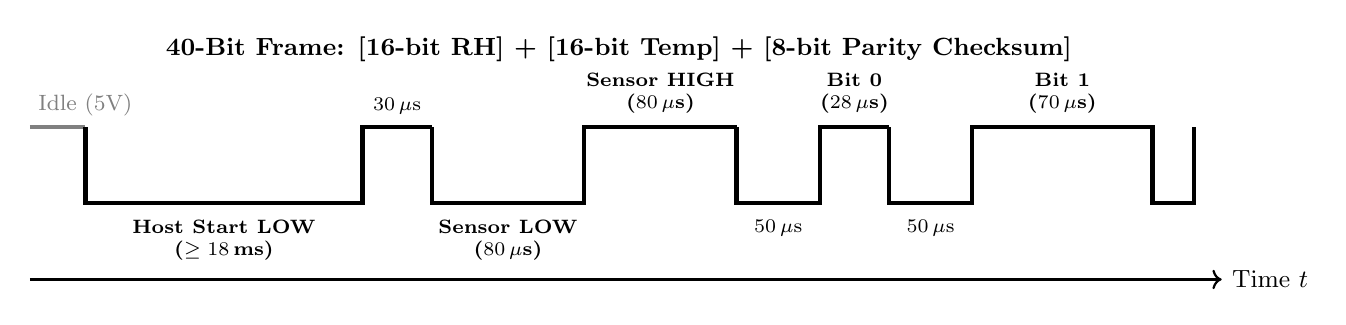
\begin{tikzpicture}[scale=0.88]
    \draw[thick, ->] (0,-0.4) -- (17.2,-0.4) node[right, font=\small] {Time $t$};
    
    % Idle State
    \draw[ultra thick, gray] (0,1.8) -- (0.8,1.8) node[above, font=\footnotesize] {Idle (5V)};
    
    % Host Start Signal (LOW >= 18ms, then HIGH 20-40us)
    \draw[ultra thick] (0.8,1.8) -- (0.8,0.7) -- (4.8,0.7) -- (4.8,1.8) -- (5.8,1.8);
    \node[below, font=\scriptsize\bfseries, align=center] at (2.8,0.6) {Host Start LOW\\($\ge 18\,\text{ms}$)};
    \node[above, font=\scriptsize] at (5.3,1.85) {$30\,\mu\text{s}$};
    
    % Sensor Response (LOW 80us, then HIGH 80us)
    \draw[ultra thick] (5.8,1.8) -- (5.8,0.7) -- (8.0,0.7) -- (8.0,1.8) -- (10.2,1.8);
    \node[below, font=\scriptsize\bfseries, align=center] at (6.9,0.6) {Sensor LOW\\($80\,\mu\text{s}$)};
    \node[above, font=\scriptsize\bfseries, align=center] at (9.1,1.85) {Sensor HIGH\\($80\,\mu\text{s}$)};
    
    % Bit 0 (LOW 50us, HIGH 28us)
    \draw[ultra thick] (10.2,1.8) -- (10.2,0.7) -- (11.4,0.7) -- (11.4,1.8) -- (12.4,1.8);
    \node[below, font=\scriptsize] at (10.8,0.6) {$50\,\mu\text{s}$};
    \node[above, font=\scriptsize\bfseries, align=center] at (11.9,1.85) {Bit 0\\($28\,\mu\text{s}$)};
    
    % Bit 1 (LOW 50us, HIGH 70us)
    \draw[ultra thick] (12.4,1.8) -- (12.4,0.7) -- (13.6,0.7) -- (13.6,1.8) -- (16.2,1.8) -- (16.2,0.7) -- (16.8,0.7) -- (16.8,1.8);
    \node[below, font=\scriptsize] at (13.0,0.6) {$50\,\mu\text{s}$};
    \node[above, font=\scriptsize\bfseries, align=center] at (14.9,1.85) {Bit 1\\($70\,\mu\text{s}$)};
    
    \node[above, font=\small\bfseries] at (8.5,2.6) {40-Bit Frame: [16-bit RH] + [16-bit Temp] + [8-bit Parity Checksum]};
\end{tikzpicture}
\caption{DHT11 Single-Bus 1-Wire Handshake and Bit Timing Sequence.}
\label{fig:dht11_timing}
\end{figure}

\subsection{Breadboard Interfacing \& Circuit Schematics}
\begin{figure}[H]
\centering
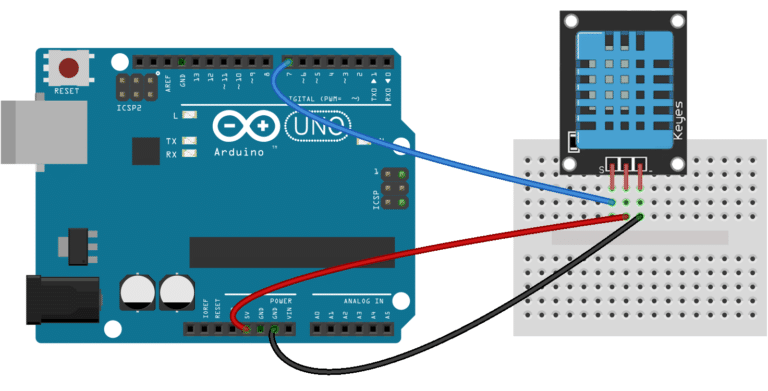
\includegraphics[height=3.8cm, keepaspectratio]{dht11_wiring.png}
\caption{Breadboard Fritzing Wiring for DHT11 Sensor Module.}
\label{fig:dht11_breadboard}
\end{figure}

\begin{figure}[H]
\centering
\begin{circuitikz}[american, scale=0.74]
    \draw[fill=white, draw=black, line width=1.0pt] (0,0) rectangle (4.2,4.0);
    \node at (2.1,3.5) [font=\bfseries\small] {ARDUINO UNO};
    
    \node (p5v) at (4.2,2.9) [anchor=east, font=\small\bfseries] {5V};
    \node (pd7) at (4.2,2.0) [anchor=east, font=\small\bfseries] {D7};
    \node (pd8) at (4.2,1.1) [anchor=east, font=\small\bfseries] {D8};
    \node (pgnd) at (4.2,0.4) [anchor=east, font=\small\bfseries] {GND};

    \draw[fill=white, draw=black, line width=0.9pt] (8.2,1.5) rectangle (11.4,3.9);
    \node at (9.8,3.4) [font=\bfseries\small] {DHT11 MODULE};
    \node (d_vcc) at (8.2,2.9) [anchor=west, font=\small] {VCC (+)};
    \node (d_dat) at (8.2,2.2) [anchor=west, font=\small] {DATA};
    \node (d_gnd) at (8.2,1.7) [anchor=west, font=\small] {GND (-)};

    \draw (4.2,2.9) -- (8.2,2.9);
    \draw (4.2,2.0) -- (8.2,2.2);
    \draw (4.2,0.4) -- (6.0,0.4) -- (6.0,1.4) -- (7.6,1.4) -- (7.6,1.7) -- (8.2,1.7);

    \draw (4.2,1.1) -- (5.0,1.1) to[R, l=$R_{\text{alert}}(220\,\Omega)$, *-] (6.8,1.1) to[leDo, -*] (8.4,1.1) -- (8.4,0.4) -- (4.2,0.4) node[ground]{};
    \node[right, font=\small\bfseries] at (8.5,1.1) {$\text{LED}_{\text{alert}}$};
\end{circuitikz}
\caption{Complete Interfacing Schematic for DHT11 Sensor and Closed-Loop Alert LED.}
\label{fig:exp3_circuit}
\end{figure}

\subsection{Pin Interconnection Table}
\begin{table}[H]
\centering
\small
\renewcommand{\arraystretch}{1.22}
\begin{tabularx}{\textwidth}{|l|l|l|X|}
\hline
\textbf{Arduino UNO Pin} & \textbf{External Component} & \textbf{Component Terminal} & \textbf{Functional Role} \\
\hline
$+5\text{V}$ & DHT11 Module & Pin 1 ($V_{CC} / +$) & Sensor DC Power Supply ($+5\text{V}$) \\
Digital Pin 7 (D7) & DHT11 Module & Pin 2 (DATA / OUT) & Bidirectional 1-Wire Telemetry Line \\
GND & DHT11 Module & Pin 3 (GND / -) & Common System Ground ($0\text{V}$) \\
\hline
Digital Pin 8 (D8) & Resistor $R_{\text{alert}}$ ($220\,\Omega$) & Lead 1 & High-Temperature Alert Output Trigger \\
Resistor $R_{\text{alert}}$ & Alert LED (Red) & Anode (Long Leg, $+$) & Current-Limited LED Driver ($I_F \approx 13.6\text{ mA}$) \\
Alert LED & Arduino GND Rail & Cathode (Flat Notch, $-$) & Ground Return Path \\
\hline
\end{tabularx}
\caption{Hardware Wiring Interconnection Matrix for Experiment 3.}
\label{tab:exp3_pins}
\end{table}

\begin{attachmentbox}
\footnotesize
\textbf{[ $\hookrightarrow$ Practical Record Attachment Reference for Experiment 3 (Complete C++ Code) ]}\\
Paste \textbf{Sheet 5 (Page 5)} from \texttt{IOT\_Printable\_Diagrams\_and\_Codes.pdf} on the \textbf{Left-Hand Blank Page} opposite this code implementation section. It contains \textbf{Program Listing 3.1} (Full Unbroken C++ Source Code).
\end{attachmentbox}

\subsection{Arduino C++ Firmware Implementation}
\begin{lstlisting}[style=bwArduino, caption={Arduino C++ Program for DHT11 Telemetry and Closed-Loop Alert Actuation.}]
/*
 * Experiment 03: DHT11 Sensor Interfacing with Closed-Loop High-Temp Alert
 * Pin Connections: DHT11 DATA -> Pin 7 | Alert Red LED -> Pin 8
 * Alarm Trigger Threshold: 30.0 deg C (Adjustable setpoint)
 */

#include <DHT.h>

#define DHTPIN 7            // DHT11 DATA connected to Digital Pin 7
#define DHTTYPE DHT11       // Sensor model designation
#define ALERT_PIN 8         // Red Alert LED connected to Digital Pin 8
#define TEMP_THRESHOLD 30.0 // Closed-loop alarm trigger setpoint in Celsius

DHT dht(DHTPIN, DHTTYPE);

void setup() {
  Serial.begin(9600);
  pinMode(ALERT_PIN, OUTPUT);
  digitalWrite(ALERT_PIN, LOW); // Initialize alert LED to OFF
  dht.begin();
  
  Serial.println("=================================================");
  Serial.println("   IoT Lab: DHT11 Telemetry & Alert System       ");
  Serial.println("=================================================");
  Serial.println("Time(s)\tHumidity(%)\tTemp(C)\tAlert Status");
}

void loop() {
  // DHT11 sampling rate is limited to 1 Hz; enforce 2.0 s polling interval
  delay(2000);

  float humidity = dht.readHumidity();
  float temperature = dht.readTemperature();

  // Validate sensor readout
  if (isnan(humidity) || isnan(temperature)) {
    Serial.println("ERROR: Failed to read from DHT11 sensor!");
    return;
  }

  // Closed-Loop Threshold Comparison Logic
  bool isAlert = (temperature >= TEMP_THRESHOLD);
  digitalWrite(ALERT_PIN, isAlert ? HIGH : LOW);

  // Stream formatted telemetry to Serial Monitor
  Serial.print(millis() / 1000);
  Serial.print(" s\t");
  Serial.print(humidity, 1);
  Serial.print(" %\t\t");
  Serial.print(temperature, 1);
  Serial.print(" C\t");
  Serial.println(isAlert ? "ACTIVE [ALERT ON]" : "NORMAL [OFF]");
}
\end{lstlisting}

\begin{attachmentbox}
\footnotesize
\textbf{[ $\hookrightarrow$ Practical Record Attachment Reference for Experiment 3 (Observations \& Output) ]}\\
Paste \textbf{Sheet 6 (Page 6)} from \texttt{IOT\_Printable\_Diagrams\_and\_Codes.pdf} on the \textbf{Left-Hand Blank Page} opposite this experimental output section. It contains \textbf{Table 3.2} (Observations Log with Modulo-256 Checksums) and the \textbf{Raw Serial Monitor Output Stream}.
\end{attachmentbox}

\subsection{Experimental Observations \& Serial Output Capture}
\begin{table}[H]
\centering
\small
\renewcommand{\arraystretch}{1.35}
\begin{tabularx}{\textwidth}{|c|p{3.2cm}|c|c|c|X|}
\hline
\textbf{S.No} & \textbf{Thermal State} & \textbf{Temp} & \textbf{Humidity} & \textbf{Alert Status ($T \ge 30^\circ\text{C}$)} & \textbf{Checksum Parity Calculation} \\
\hline
1 & Ambient Lab Environment & $27.4^\circ\text{C}$ & $62.0\%$ & \textbf{OFF (Normal)} & $\text{0x1B} + \text{0x00} + \text{0x3E} + \text{0x00} = \text{0x59}$ [PASS] \\
2 & Ambient Lab Environment & $28.1^\circ\text{C}$ & $60.5\%$ & \textbf{OFF (Normal)} & $\text{0x1C} + \text{0x00} + \text{0x3C} + \text{0x00} = \text{0x58}$ [PASS] \\
3 & Elevated Heat Applied & $31.8^\circ\text{C}$ & $74.0\%$ & \textbf{ON (ACTIVE ALERT)} & $\text{0x1F} + \text{0x00} + \text{0x4A} + \text{0x00} = \text{0x69}$ [PASS] \\
4 & Peak Heated State & $34.0^\circ\text{C}$ & $86.0\%$ & \textbf{ON (ACTIVE ALERT)} & $\text{0x22} + \text{0x00} + \text{0x56} + \text{0x00} = \text{0x78}$ [PASS] \\
5 & Post-Cooling Normal & $28.5^\circ\text{C}$ & $65.0\%$ & \textbf{OFF (Normal)} & $\text{0x1C} + \text{0x00} + \text{0x41} + \text{0x00} = \text{0x5D}$ [PASS] \\
\hline
\end{tabularx}
\caption{Measured Environmental Telemetry and Closed-Loop Alert Evaluation Log.}
\label{tab:exp3_log}
\end{table}

\begin{lstlisting}[style=bwTerminal, caption={Raw Serial Monitor Output Stream (9600 Baud).}]
=================================================
   IoT Lab: DHT11 Telemetry & Alert System       
=================================================
Time(s)	Humidity(%)	Temp(C)	Alert Status
2 s	62.0 %		27.4 C	NORMAL [OFF]
4 s	60.5 %		28.1 C	NORMAL [OFF]
6 s	74.0 %		31.8 C	ACTIVE [ALERT ON]  <-- [Thermal Stimulus Applied]
8 s	86.0 %		34.0 C	ACTIVE [ALERT ON]  <-- [Peak Heating Condition]
10 s	65.0 %		28.5 C	NORMAL [OFF]       <-- [Normalized Below 30 C]
\end{lstlisting}

\subsection{Discussion \& Error Analysis}
\begin{itemize}[noitemsep]
    \item \textbf{Sampling Rate Constraints:} The DHT11 internal processing cycle takes $\approx 1.0\,\text{s}$. Polling faster than $1\,\text{Hz}$ causes the sensor to return stale measurements or generate parity checksum errors.
    \item \textbf{Open-Drain Bus Requirements:} The bidirectional DATA line requires an external pull-up resistor ($4.7-10\,\text{k}\Omega$) to prevent the bus from floating when neither the MCU nor the DHT11 is pulling the line LOW.
    \item \textbf{Closed-Loop Hysteresis Control:} In real-world thermal applications, a hysteresis band (e.g., ON at $30.0^\circ\text{C}$, OFF at $28.5^\circ\text{C}$) prevents rapid mechanical or relay oscillation (chattering) around the threshold boundary.
\end{itemize}

\subsection{Viva-Voce Questions \& Detailed Answers}
\begin{enumerate}[leftmargin=*]
    \item \textbf{Q: How does the DHT11 represent logic `0` versus logic `1`?}\\
    \textbf{Ans:} Both bit transmissions start with a $50\,\mu\text{s}$ LOW pulse. The subsequent HIGH duration distinguishes the bit: a $26-28\,\mu\text{s}$ HIGH duration represents logic `0`, whereas a $70\,\mu\text{s}$ HIGH duration represents logic `1`.
    \item \textbf{Q: What is the mathematical formula used to verify the DHT11 parity checksum?}\\
    \textbf{Ans:} $\text{Checksum Byte} = (\text{Byte 1} + \text{Byte 2} + \text{Byte 3} + \text{Byte 4}) \pmod{256}$. If the received fifth byte equals the lower 8 bits of the sum of the preceding four data bytes, the transmission is valid.
    \item \textbf{Q: What causes `NaN` (Not a Number) errors in Arduino DHT library readings?}\\
    \textbf{Ans:} A `NaN` error occurs when the sensor fails to respond to the host start signal within the expected $80\,\mu\text{s}$ window, when a transmission timeout occurs, or when the 8-bit parity checksum validation fails due to wiring noise.
\end{enumerate}

\newpage

% ==============================================================================
% REFERENCES & STANDARDS
% ==============================================================================
\section{Engineering Standards \& Reference Documentation}
\begin{enumerate}[noitemsep]
    \item ITU-T Recommendation Y.2060 (06/2012): \textit{Overview of the Internet of Things}, International Telecommunication Union.
    \item IEEE Standard 802.15.4-2020: \textit{Low-Rate Wireless Networks}, IEEE Computer Society.
    \item OASIS Standard: \textit{MQTT Version 3.1.1 Specification}, OASIS Message Queuing Telemetry Transport Technical Committee.
    \item IETF RFC 7252 (2014): \textit{The Constrained Application Protocol (CoAP)}, Internet Engineering Task Force.
    \item Microchip Technology: \textit{ATmega328P 8-bit AVR Microcontroller Datasheet} (DS40002061B).
    \item Aosong Electronics: \textit{DHT11 Digital-output relative humidity \& temperature sensor/module Datasheet}.
\end{enumerate}

\end{document}
